\chapter{Methods}
\label{chp:methods}
% ------------------------------------------------------------------------------

% CHAPTER INTRODUCTION
% * what is discussed in this chapter?
% * emulation is discussed, with focus in hydrology
% * introduce the tools needed for emulation: they will be explained later
%   in detail
% * simulation is used to explore
% * experiment: we mean here numerical experiment -> say it!



In this chapter we give an introduction about emulation.
We explain what it is, how it works, and what it needs.
We then propose a workflow to follow in order to implement it.

We then present the tools and the methods required and briefly describe them
The tools used for the scope of this thesis are then presented and described.



%Unlike high performance computing (HPC), emulation is one way of reducing computational time with no big investments.




% ==============================================================================
\section{Emulation}
% ==============================================================================
%-------------------------------------------------------------------------------
%If you do not cleanly separate into Methods and Material, you have to say at one point what you present where. This can either be done after research questions (the structure of the thesis is as follows: first, ... second). or here. To guide the reader.

%After Emulation description: 

%In the following, I will first describe introduce mechanistic emulators/compare the concept of mechanistic /phenomenological emulators with a didactical case study. Second, use emulators in a practically relevant task: time-to-threshold, i.e. time until sounding flood alarm. 

%The first example is continuous => straightforward. the second is more complex => classification of input/output space. => hierarchical emulator?
%-------------------------------------------------------------------------------

% * explain emulation more in detail (present schemes JPi)
% * give emulation examples?
% * add a scheme with the workflow for emulation!
% * see https://www.intechopen.com/source/html/43001/media/image27.png
%   for example workflow/pseudocode
% * emulating: approximation model of a detailed simulator
% * loss of information and accuracy
% * probe
% * emulator not replacing simulator. It replace one or some of the tasks done
%   by the simulator
% * emulation in hydrodynamic very interesting: simulators solve PDE over
%   complex domains (slow). 
% * prior knowledge from the PDEs can be encoded in GP
% * emulators are task-specific
% * speedup gain at the expenses of information/accuracy
% * emulators scarify unneeded accuracy in favor of speed (Carbajal, 2017)







\seb{I really don't know how to begin this section...}
The big advantages offered in terms of costs, the increasing performance of computers and the growing variety of task that can be tackled with, has lead to spreading of simulation to diverse sectors of science and engineering \autocite{gorissen_surrogate_2010}.
Simulators have become more accurate, their level of detail has grown, allowing in some cases for the replacement of classical physical experiments.
However, the widespread exploitation of simulation has increased the awareness of its main drawback: the considerable computational cost of these high fidelity simulators.
A possible solution to the problem is the use of emulators, approximation models reproducing the behaviour of the detailed simulator.
With the construction of emulators, huge speedups can be achieved; these at the expenses of unneeded detail and accuracy \autocite{carbajal_appraisal_2016}.

Details are sacrificed with the construction of emulators. Emulators are task-specific, they are built to answer a specific question: if the question changes, a new, ad hoc emulator have to be built.
Let us make an example from the hydrodynamics field.
We can imagine extracting time-series of water depth at a specific point in a river channel from hydrodynamical simulations.
The simulation inputs are different hydrographs, the outputs are the time-series generated by the hydrographs.
An emulator can be built for this task, predicting the pattern of the water depth time-series as a function of the input hydrograph given.
Now, if the focus changes, and we are suddenly interested in the pattern of the flow velocity time-series at that point, we can simply extract it from the simulations.
The emulator however, has no knowledge of the flow velocity.
It was built and trained with water depth data and it cannot in any way make flow velocity predictions.
If the task has to be accomplished many times, it could make sense to build a new emulator for this.

Not only information about other variables, not directly linked with the one studied are lost by building an emulator.
Emulators can be space-specific (e.g. water depth time-series at a specific point) or time specific (e.g. water depth profile along a channel at specific instant).
When obtaining these information from a detailed hydrodynamical simulator, the simulator goes through a series of \emph{internal states} that we do not really need for our application.
A Finite Element Method (FEM) simulator for example, has to solve the SWE over the whole grid, although the output we are interested in is just the water depth at the chosen point.
Here the internal states are represented by the solution of the SWE at every grid cell, whereas our output, the information we are interested in, is the water depth at the chosen location.
The structure of such simulators is said "fan-out/fan-in" \autocite{carbajal_emumore_2017}. A schematic representation of this structure can be observed in Fig.~\ref{fig:simulation}.

\begin{figure}[h]
  \centering
  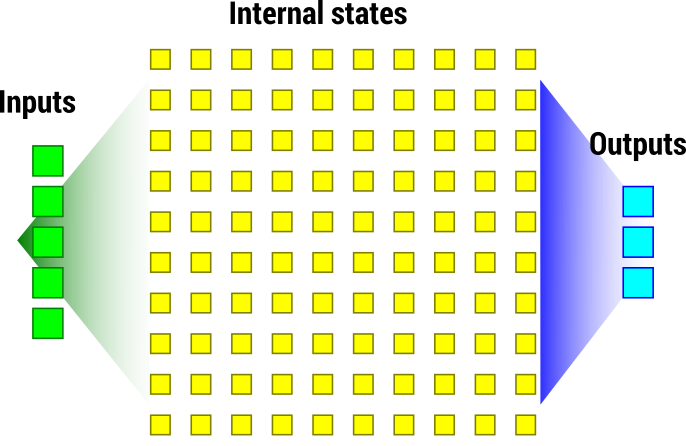
\includegraphics[width=0.7\textwidth]{Figures/simulation.png}
  \caption{Fan-out/fan-in structure of typical simulators used in hydrodynamics, solving the SWE over a grid \autocite{carbajal_emumore_2017}.}
  \label{fig:simulation}
\end{figure}

In contrast with simulators, emulators bridge the internal states: it goes from inputs to desired output directly, without passing through the internal states.
The emulator establishes a direct functional relationship between inputs and output.
It \emph{learns} this relationship from corresponding inputs-output sets.
Once the relationship is learned, and the model is validated, our emulator is ready to be exploited: it can now produce output predictions for new input values.
Fig.~\ref{fig:emulation} depicts this relationship bridging the internal states.

\begin{figure}[h]
  \centering
  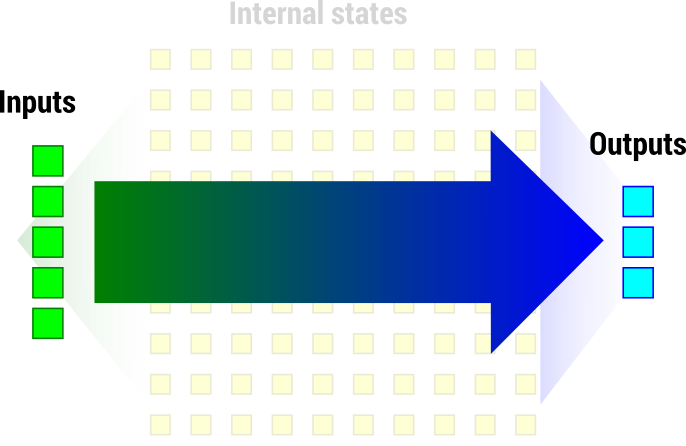
\includegraphics[width=0.7\textwidth]{Figures/emulation.png}
  \caption{Emulator functioning: a direct relationship linking the inputs to the outputs, independent from the internal states \autocite{carbajal_emumore_2017}.}
  \label{fig:emulation}
\end{figure}

The data needed for learning this relationship are inputs-output sets.
These are obtained by sampling the input space within the range needed with an appropriate technique, depending on the amount of input variables our problem has.
With every inputs-set a simulation is run and the desired output is extracted, generating this way our dataset.
The relationship has then to be learned with an appropriate technique: building an emulator is a regression problem, even more, it is an interpolation problem \autocite{carbajal_emumore_2017} which can be addressed with modern ML methods.\\

Emulators can mainly be divided into two groups: \emph{mechanistic} emulators and purely \emph{data-driven} emulators.
The first ones are built with methods able to encode prior knowledge of the system, introducing conditions guiding and constraining the interpolation problem.
The second ones, exploit techniques that blindly uncover relationships within the data, with no knowledge about the process generating them.
Whether to use a mechanistic or a purely data driven emulator is often quite subjective; studies try however to give guidelines helping with this choice \autocite{carbajal_appraisal_2016}.

\seb{ideal would be to introduce a workflow for implementing emulation}


% ------------------------------------------------------------------------------
\section{Regression and interpolation methods}
% ------------------------------------------------------------------------------
% * explain the terminology: interpolation, INTRAPOLATION, extrapolation
% * put it as subsection only if there is 2.2.2, otherwise just 2.2
% * explain the work done on regression and interpolation
% * explain their relation with emulation
% * cite James et al., 2013 -> learning from data or predict outputs

Key step when building an emulator is establishing the inputs-output relationship, namely solve the regression/interpolation problem.
For this many different methods exist; which one to choose may depend on the dimensions of the inputs space, the availability of data, the previous knowledge about the considered system, and weather we want to make predictions or learning functional relationships from our data.

Usually, when learning functional relationships from physical experimental data, we are trying to solve a regression problem.
The observation we are using are subject to errors assumed to be independent and Gaussian distributed due to the stochasticity of the problem.
Since the observation does not represent necessarily the true value, we then perform a regression, e.g. using the least squares (LS) method, minimizing the sum of squared residuals.
In this thesis, 



% ==============================================================================
\section{Simulation in hydrodynamics}
% ==============================================================================
% * transfer functions
% * PDEs
% * https://en.wikipedia.org/wiki/Routing_(hydrology)
% * go for hydrodynamic simulation => more detailed, more complex, slower
% * (Hydrological models could even be considered "emulators" of the more
%   detailed PDE-simulators)



% ------------------------------------------------------------------------------
\subsection{FullSWOF\_2D-v1.07.00}
% ------------------------------------------------------------------------------
% * show the results of a simulation (cross-reference with channel simulation)
% * 


The simulator chosen to produce the datasets for the later emulation task is \citetalias{delestre_fullswof:_2017}. FullSWOF (Full Shallow Water equations for Overland Flow) is an \emph{open source} software solving the Shallow Water equations using finite volumes and methods especially chosen for hydrodynamic purposes \autocite{the_fullswof_team_fullswof_2018}.\\

In order to run simulations the software needs at least the following inputs:

\begin{itemize}
\itemsep0em
  \item a \emph{parameters file}
  \item a \emph{topography file}
  \item an \emph{initial conditions file}
\end{itemize}

\paragraph{Parameters file} A text file defining the values set for all of the simulation parameters. This can be generated with the function \textit{params2file} of the fswof2d package, where to every parameter a default value is already given and only parameter values different from the default ones have to be modified. Simulation parameters include:

\begin{itemize}
\itemsep0em
  \item Number of cells (x and y directions)
  \item Simulation duration
  \item Number of intermediate states saved
  \item Domain length
  \item Domain width
  \item Boundary conditions specifications
  \item Various settings for the numerical schemes
  \item Different physical parameters (friction coefficient, initial soil saturation, soil thickness, soil hydraulic conductivity, maximal infiltration)
\end{itemize}

The physical parameters are spatially distributed. A unique value for the whole domain can be used or a value for every cell can be defined by giving to the simulator a text file specifying all of the values.\\

Output is written to five different \emph{output files}.
To one file only the initial state (at $t = \SI{0}{\s}$) of the simulation is written.
This corresponds to the initial conditions file.
To a second file the final state of the simulation is saved (at $t = t_{max}$).
A third file stores the whole evolution of the simulation: it begins with the initial conditions and ends with the final state.
In between the intermediate results are stored.
How many intermediate results to saved is set by the user in the parameters file.
The fourth file stores the information relative to the water budget.
How much water was lost through the boundaries, how much infiltrated and how much is present over the topography.
The fifth is just a copy of the parameters file.
It is useful to know which parameters were set to generate the given output.

\paragraph{Topography file} FullSWOF\_2D solves the Shallow Water equation over a regular uniform grid. The computational domain is therefore a rectangle and the cells composing it are rectangles too, all with the same size. The topography file is a text file specifying the x,y,z coordinates of the center of every cell.

\paragraph{Initial conditions file} A text file defining the initial conditions of the simulation. It specifies the \emph{water depth}, the \emph{flow velocity in x} and the \emph{flow velocity in y} for all cells of the domain. All of these can also be set to \num{0}.\\

Water can enter the domain through the boundaries (\emph{imposed discharge}) or with the rain. If the option rain is chosen, a \emph{rain file} has to be provided. This defines the hyetograph of the rain event, the rain intensity as a function of time. The rain is uniformly applied to the domain.


% ------------------------------------------------------------------------------
\subsection{Development of \textit{FullSWOF\_2D} interaction tools}
\label{sec:fswof_interaction_tools}
% ------------------------------------------------------------------------------
% FULLSWOF2D PACKAGE
% * list the functions developed
% * high-level infos what functions do
%   - input
%   - output
%   - methods/operations
% * or move to appendix if no time
% * put just summary in main body:
%   "fswof2d has 18 functions with 20 methods to convert data, pre-processes
%    grids for efficient construction of simulation domain, interface Octave
%    engine (see Appendix X for details.)"



As already mentioned in section \seb{mention which section} \textit{FullSWOF\_2D-v1.07.00} was chosen as \emph{overland flow simulator} in order to generate the required datasets.
\textit{FullSWOF\_2D} needs at least three input files in order to run simulations:

\begin{itemize}
\itemsep0em
  \item \textit{topography}: a text file specifying the topography of the domain
  \item \textit{parameters}: a text file specifying the values set for the simulation parameters
  \item \textit{huv\_init}: a text file defining the initial conditions of the problem (initial water height and initial water velocity at every point of the grid)
\end{itemize}

In order to generate these files, interaction functions were developed with the open source tool \textit{Octave 4.2.1} \autocite{octave_community_gnu_2018}.
The interaction functions were grouped into the Octave package \textit{fswof2d} available at \url{https://bitbucket.org/binello7/fswof2d}.\\

The package includes the following functions, all of which are distributed under \textit {GPLv3} license \autocite{smith_quick_2014}.

\begin{itemize}
\itemsep0em
  \item center2node.m
  \item csec\_channel2lvlsym.m
  \item dataconvert.m
  \item extrude\_csec.m
  \item huv2file.m
  \item matplotlib\_cm.m
  \item node2center.m
  \item params2file.m
  \item read\_params.m
  \item topo2file.m
\end{itemize}



\textit{FullSWOF\_2D} uses a regular uniform grid in order to solve the \emph{shallow water equation} with the finite volume method (FVM).
The equations are solved at the center of every cell.
After creating the vector defining the grid nodes, one can use the \textit{center2node} function to compute the centers of the grid cells.
This is particularly useful because the $(x,y)$ coordinates saved to the \textit{topography} file have to be the coordinates of the cell centers.
A short usage example would be:







